\documentclass{beamer}

% ////////////////////////////////////////////////////////////////////////////
% Instructions for authors
% ////////////////////////////////////////////////////////////////////////////
% 
% Please scan the current document and notices how it is divided into sections
% Only one author per slide, please! This will reduce merge conflicts
% Create new commands in separate sections marked by your initials
% The document width is 78 characters.

% Configuration of beamer
\usetheme{Copenhagen}
\setbeamertemplate{navigation symbols}{}
\setbeamertemplate{footline}[frame number]

% Basic packages
\usepackage{graphics,graphicx,hyperref,amsmath,amssymb,amsthm,color,multirow}
\usepackage{ragged2e}
\usepackage{verbatim,listings}
\usepackage[normalem]{ulem}
\usepackage{hhline}
% Set the graphics path
% \graphicspath{{./graphics/people/}{./graphics/logos/}}

% ////////////////////////////////////////////////////////////////////////////
% LaTeX shortcut commands typically defined by CCKM
% ////////////////////////////////////////////////////////////////////////////

% Theorems
\newtheorem{algorithm}[theorem]{Algorithm}

% Finite dimensional vectorspaces
\newcommand{\R}{\mathbb{R}}
\newcommand{\Rn}{\R^n}
\newcommand{\Rp}{\R^p}
\newcommand{\Rnn}{\R^{n \times n}}
\newcommand{\Rnp}{\R^{n \times p}}
\newcommand{\myspan}{\text{span}}

% Equations
\newcommand{\be}{\begin{equation}}
  \newcommand{\ee}{\end{equation}}
\newcommand{\bes}{\begin{equation*}}
  \newcommand{\ees}{\end{equation*}}

% Matrices
\newcommand{\bbm}{\begin{bmatrix}}
  \newcommand{\ebm}{\end{bmatrix}}
\newcommand{\bpm}{\begin{pmatrix}}
  \newcommand{\epm}{\end{pmatrix}}

% Sets
\newcommand{\Ran}{\text{Ran}\:}
\newcommand{\Ker}{\text{Ker}\:}

% Floating point representation
\newcommand{\fl}{\text{fl}}

% ////////////////////////////////////////////////////////////////////////////
% Specialized graphics
% /////////////////////////////////////////////////////////////////////////// 

\usepackage{tikz}
\usetikzlibrary{shapes}
\setbeamerfont{block title}{size=\small}

\title[Introduction to HPC2N]{Introduction to HPC2N}
%\subtitle{}
%\author{Birgitte Bryds\o, Mirko Myllykoski, and Pedro Ojeda-May}
\author{Birgitte Bryds\o, Pedro Ojeda-May}
\institute{HPC2N, Ume\aa{} University}

\titlegraphic{\center{
\includegraphics[height=1.2cm]{figures/naiss.png}\hspace*{1.1cm}~
   
\includegraphics[height=1.2cm]{figures/umu-logotyp-EN.png}\hspace*{1.1cm}~
\includegraphics[height=1.2cm]{figures/hpc2n.png}
}}
\date{18 January 2024}
\begin{document}

\frame{
  \titlepage
}


\frame{\frametitle{Overview}

  \begin{block}{}
\begin{itemize}
\item Projects - compute and storage 
\item Using our systems
\item The File System 
\item The Module System
 \begin{itemize}
  \item Overview 
  \item Compiler Tool Chains
  \item Examples
 \end{itemize}
\item Compiling/linking with libraries 
\item The Batch System (SLURM)
 \begin{itemize}
\item Overview 
\item Examples
 \end{itemize}
\end{itemize}
  \end{block}

}


\frame{\frametitle{Projects - compute and storage}
  \begin{small}
    Join a project or apply for one. 
  \end{small}
  \begin{block}{}
      \begin{itemize}
    \begin{footnotesize}
      \item Kebnekaise is only open for local project requests.
        \begin{itemize}
          \begin{footnotesize}
          \item The PI must be affiliated with UmU, LTU, IRF, MiUN, or SLU.
          \item You can still add members (join) from anywhere.
          \end{footnotesize}
        \end{itemize}
      \item Apply for \textbf{compute project} in SUPR \texttt{https://supr.naiss.se/round/compute}
        \begin{itemize}
          \begin{footnotesize}
          \item Login to SUPR (create SUPR account if you do not have one).
          \item Click “Rounds” in the left menu. Pick “Compute Rounds”. Pick “Centre Local Compute”.
          \item Pick “HPC2N Local Compute YYYY”. Choose “Create New Proposal for HPC2N Local Compute YYYY”.
          \item Create from scratch or use earlier proposal as starting point.
          \item Agree to the default storage if 500GB is enough. 
          \item More information: \\
            \begin{scriptsize}
              \texttt{https://supr.naiss.se/round/open\_type/?type=Centre+Local+Compute}
            \end{scriptsize}
          \end{footnotesize}
        \end{itemize}
      \item If the above mentioned default storage is not enough, you will need to apply for a \textbf{Local storage project}: \\
        \begin{scriptsize}
          \texttt{https://supr.naiss.se/round/open\_type/?type=Centre+Local+Storage}
        \end{scriptsize}
    \end{footnotesize}
      \end{itemize}
  \end{block}
}

\frame{\frametitle{Projects - compute and storage}

  \begin{block}{}
    \begin{itemize}
    \item As default, you have 25GB in your home directory.
    \item If you need more, you/your PI can accept the ``default storage''
      you will be offered after applying for compute resources.
    \item The default storage is 500GB.
    \item If you need more than that, you/your PI will have to apply for a
      storage project.
    \item When you have both, link them together. It is done from the \textbf{storage} project. 
    \end{itemize}
  \end{block}

}

% \frame{\frametitle{Projects - compute and storage}

%     After indicating the amount of compute resources you want, you
%     will be asked if you want the default amount of storage:
%   \begin{block}{}
% 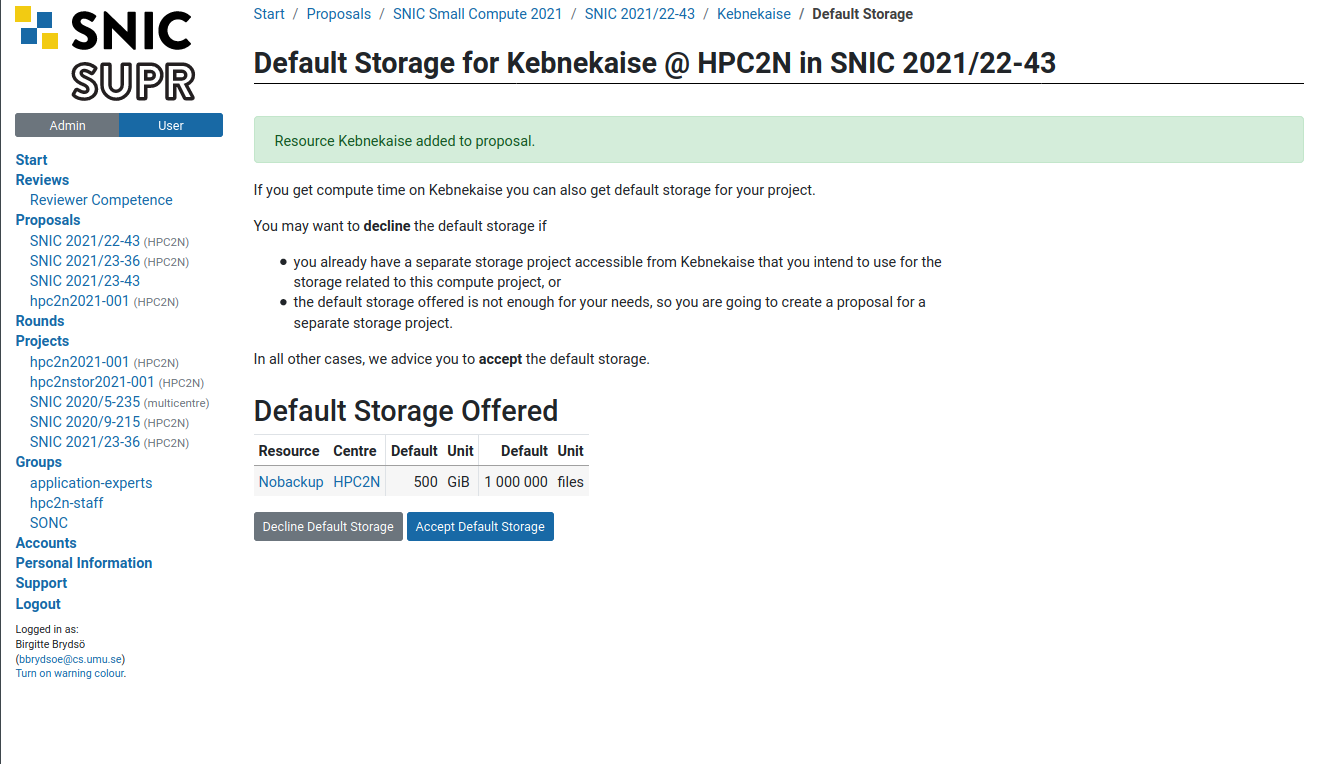
\includegraphics[height=7cm]{figures/default-storage.png}
%   \end{block}

% }

% \frame{\frametitle{Projects - compute and storage}

%     You will also be asked what the default storage directory should
%     be called: 
%   \begin{block}{}
% 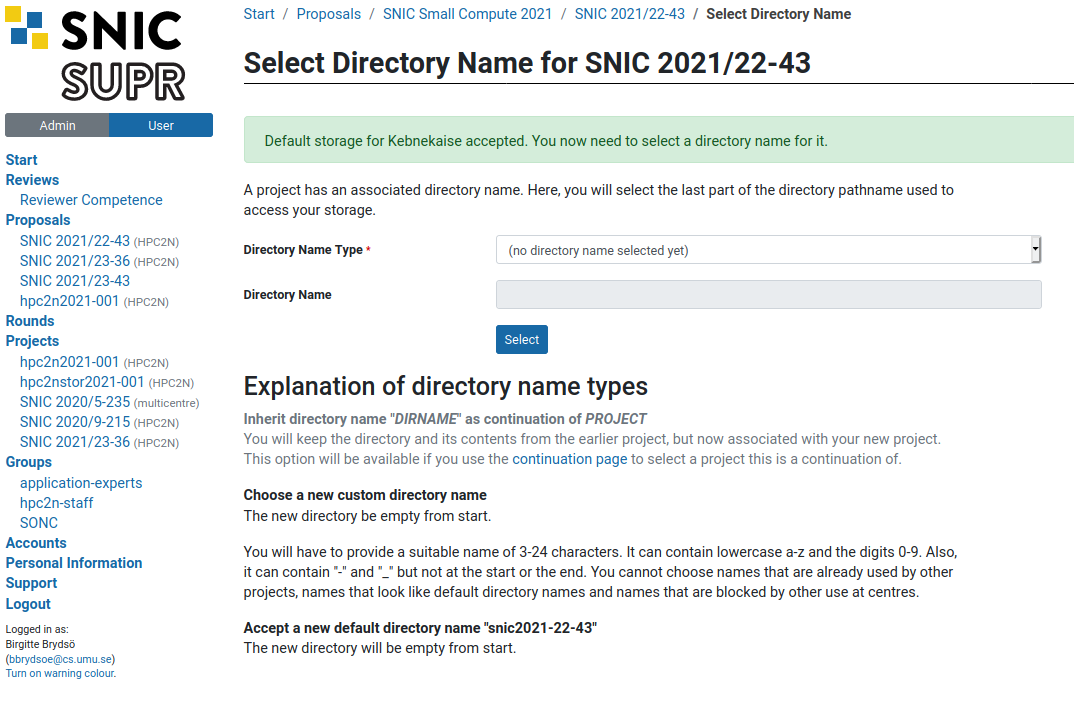
\includegraphics[height=7cm]{figures/default-dir.png}
%   \end{block}

% }

\frame{\frametitle{Projects - compute and storage}

  \begin{block}{}
    \begin{itemize}
    \item After applying on SUPR, the project(s) will be reviewed.
    \item When (if) the projects are approved, the PI needs to link
      the compute and storage projects together if they applied for
      both.
    \item Linking them together is done from the \textbf{storage} project. 
    \item This way all members of the compute project also becomes
      members of the storage project.
    \end{itemize}
  \end{block}

}

\frame{\frametitle{Projects - compute and storage}

    Linking a compute project to a storage project:
  \begin{block}{}
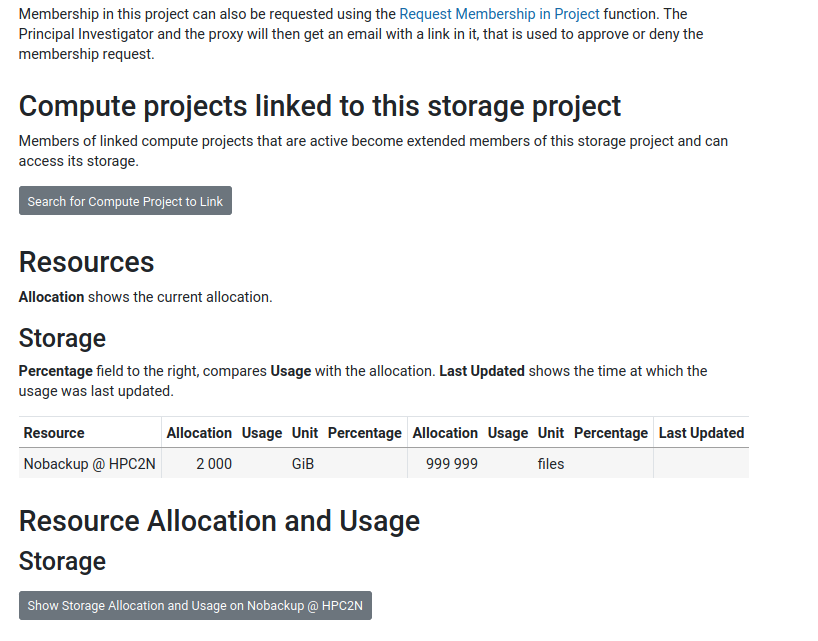
\includegraphics[height=7cm]{figures/to-link.png}
  \end{block}

}

\frame{\frametitle{Projects - compute and storage}

  Pick a compute project to link:
  \begin{block}{}
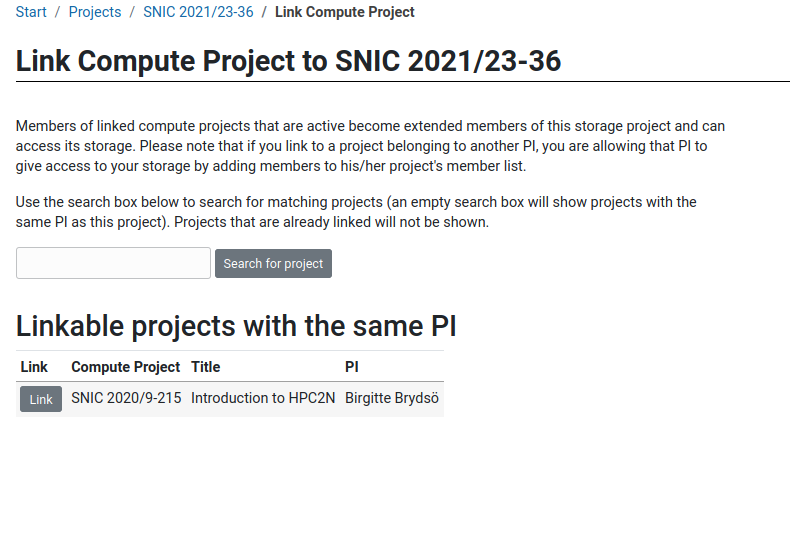
\includegraphics[height=7cm]{figures/choose2.png}
  \end{block}

}

\frame{\frametitle{Projects - compute and storage}

  Showing linked projects:
  \begin{block}{}
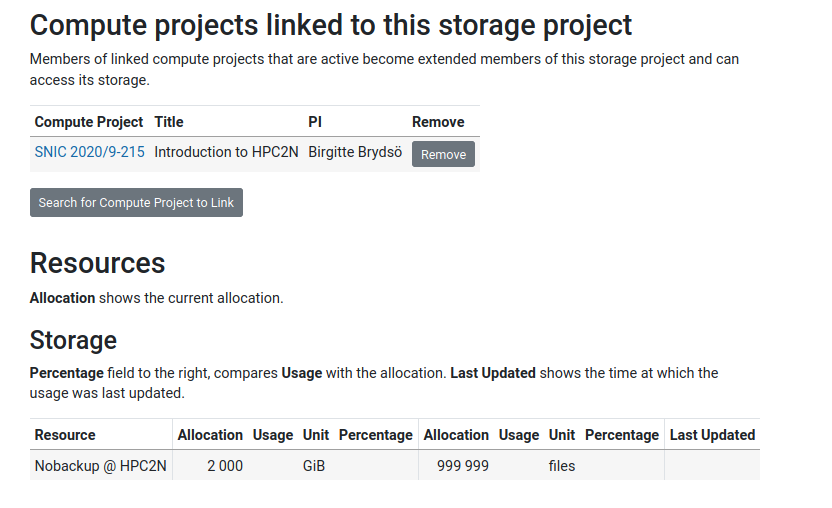
\includegraphics[height=7cm]{figures/linked.png}
  \end{block}

}

\frame{\frametitle{Projects - compute and storage}

  Members of the storage project after linking:
  \begin{block}{}
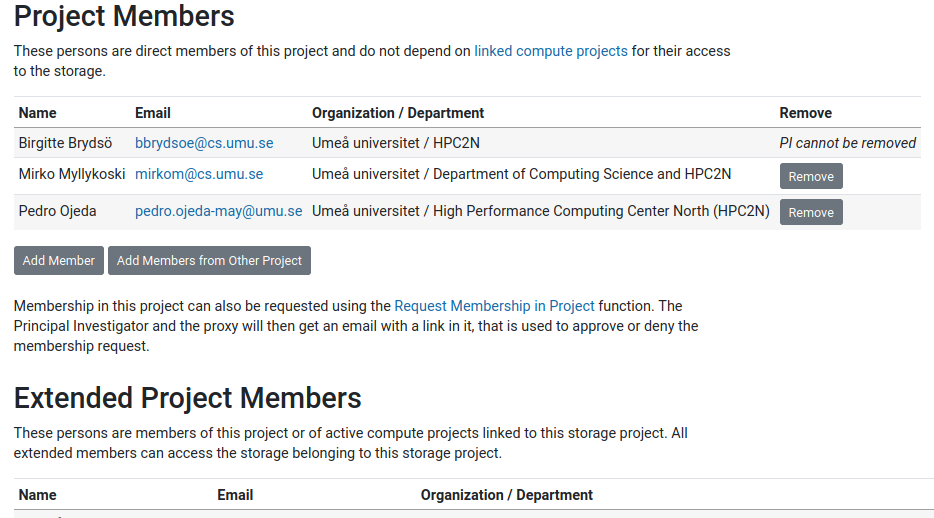
\includegraphics[height=6.5cm]{figures/storage-members.png}
  \end{block}

}

% \frame{\frametitle{Projects - after 2022-12-31?}

%   \begin{block}{}
%     \begin{itemize}
%     \item Nothing known for sure yet, but hopefully it will be clearer in a few weeks.
%     \item Non-UmU PI: You can continue working at Kebnekaise until 2022-12-31, but you should be prepared for the situation where you will have to migrate to another centre. 
%     \item Hopefully Kebnekaise will at least exist as a local resource after the new year, until it can be replaced with a newer suitable resource.
%     \item Local (UmU) PIs who have a need of using Kebnekaise (or another HPC2N resource) are encouraged to voice this to the people at UmU with the power to influence this.
%     \end{itemize}
%   \end{block}

% }

\frame{\frametitle{Using our systems - example process}

  \begin{block}{}
    \begin{enumerate}
%    \item Get an account \tiny{(https://www.hpc2n.umu.se/documentation/access-and-accounts/users)} \normalsize{}
    \item Connect to Kebnekaise:
      \begin{itemize}
      \item \textbf{ThinLinc: \texttt{kebnekaise-tl.hpc2n.umu.se}}
        \item ThinLinc through a browser (less features): \\
          \vspace{1mm}
          \texttt{https://kebnekaise-tl.hpc2n.umu.se:300/}
          \vspace{1mm}
        \item SSH: \texttt{kebnekaise.hpc2n.umu.se}
          \item \textbf{A100 or AMD Zen3}: \texttt{kebnekaise-amd-tl.hpc2n.umu.se} or \texttt{kebnekaise-amd.hpc2n.umu.se}
        \end{itemize}
      \item Transfer your files and data (if needed)
      \item Load modules (if needed)
      \item Compile own code, install software, or run pre-installed software 
      \item Create batch script, submit batch job
      \item Download data/results to local/other machine (optionally)
      \end{enumerate}
    \end{block}
    
  }

\frame{\frametitle{Using our systems}\framesubtitle{Connecting to HPC2N's systems - ThinLinc}

  \begin{small}
  \begin{block}{}
ThinLinc: a cross-platform remote desktop server from Cendio AB. Especially useful when you need software with a graphical interface.
  \end{block}{}
      \end{small}

  \begin{block}{}
    \begin{small}
      \begin{itemize}
	      \item We \textbf{recommend} ThinLinc if you don't have a preferred SSH client.
      \item Download the client from \texttt{https://www.cendio.com/thinlinc/download}. Install it.
      \item Start the client. Enter the name of the server: \textbf{kebnekaise-tl.hpc2n.umu.se}. Enter your username. 
      \item Go to "Options" $->$ "Security". Check that authentication method is set to password.
      \item Go to "Options" $->$ "Screen". Uncheck "Full screen mode".
      \item Enter your HPC2N password. Click "Connect"
      \item Click "Continue" when you are being told that the server's host key is not in the registry. Wait for the ThinLinc desktop to open.
      \end{itemize}
      \end{small}
  \end{block}

}

\frame{\frametitle{Using our systems}\framesubtitle{Transfer your files and data}

  \begin{block}{}
    \begin{itemize}
    \item \textbf{Linux, OS X:} 
    \begin{itemize}
       \item Use scp for file transfer:\\
\vspace{2mm}
\begin{footnotesize}
\texttt{local> scp username@kebnekaise.hpc2n.umu.se:file .}\\
\texttt{local> scp file username@kebnekaise.hpc2n.umu.se:file}
\end{footnotesize}
    \end{itemize}
    \item \textbf{Windows:} 
    \begin{itemize}
       \item Download client: WinSCP, FileZilla (sftp), PSCP/PSFTP, ...
       \item Transfer with sftp or scp
    \end{itemize}
       \item \scriptsize{https://www.hpc2n.umu.se/documentation/filesystems/filetransfer} \normalsize{}
    \item \textbf{Mac/OSX:}
    \begin{itemize}
       \item Transfer with sftp or scp (as for Linux) using Terminal
       \item Or download client: Cyberduck, Fetch, ...
    \end{itemize}
       \item More info in guides (see previous slide) and here: \scriptsize{https://www.hpc2n.umu.se/documentation/filesystems/filetransfer} \normalsize{}
    \end{itemize}
  \end{block}

}


 \frame{\frametitle{Using our systems}\framesubtitle{Editors}

  \begin{block}{}
    \justify
    Editing your files
  \end{block}

  \begin{block}{}
\begin{itemize}
\item Various editors: vi, vim, nano, emacs ...
\item Example, nano:
 \begin{itemize}
 \item \texttt{nano $<$filename$>$}
 \item Save and exit nano: \texttt{Ctrl-x}
 \end{itemize}
\item Example, Emacs: 
 \begin{itemize}
 \item Start with: emacs
 \item Open (or create) file: Ctrl-x Ctrl-f
 \item Save: Ctrl-x Ctrl-s
 \item Exit Emacs: Ctrl-x Ctrl-c
 \item (If you want to run in an a separate emacs window, and with
   full functionality, you need to login with ThinLinc, ssh -Y or
   similar, for X11 forwarding) 
 \end{itemize}
\end{itemize}
  \end{block}
}

\begin{frame}[fragile]
  \frametitle{Using our systems}\framesubtitle{Editors - nano}

  \begin{block}{}
    \justify
    Editing your files with nano
  \end{block}

  \begin{block}{}
     \begin{itemize}
     \item Starting “nano”: Type nano FILENAME and press Enter.
     \item If FILENAME exists, it will open, otherwise it will be created.
     \item 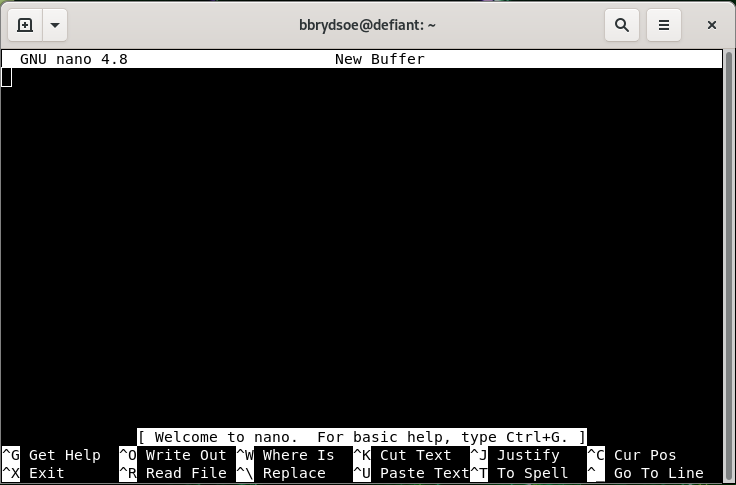
\includegraphics[height=2.5cm]{figures/nano.png}
     \item Notice: many of the commands are listed at the bottom.
     \item $\hat{\, }$ before a letter-command means press CTRL + the letter.
%     \item Your prompt is in the editor window. You can directly type content in your file.
     \item To exit (and possibly save), press CTRL + x (this is written CTRL-x or $\hat{\, }$x). nano asks if you want to save before exiting.
 \end{itemize}
  \end{block}
\end{frame}

\frame{\frametitle{The File System}

   \begin{block}{}
     \justify
     More info here: http://www.hpc2n.umu.se/filesystems/overview
   \end{block}

%      \renewcommand*{\arraystretch{1.5}}
   \begin{block}{}
    \begin{scriptsize}
      \begin{tabular}{|c|c|c|c|}
     \hline
     & & & \\ 
        & \textbf{Project storage} & \textbf{\$HOME} &
                                                       \textbf{/scratch} \\
        & & & \\ \hhline{|=|=|=|=|} 
     Recommended & & & \\
	      for batch jobs & Yes & No (size) & Yes \\ \hline 
     Backed up & No & Yes & No \\ \hline 
     Accessible & & & \\
     by batch & Yes & Yes & Yes (node only) \\ 
     system & & & \\ \hline 
     Performance & High & High & Medium \\ \hline 
     Default & & & \\
     readability & Group only & Owner & Owner \\ \hline 
     Permissions & & & \\ 
     management & chmod, chgrp, ACL & chmod, chgrp, ACL & N/A for
                                                          batch jobs \\ \hline 
     & Storage your group & & \\
     Notes & get allocated through & Your home- & Per node \\
     & the storage projects & directory & \\
     \hline
   \end{tabular}
   \end{scriptsize}
     \end{block}

   }
   
\frame{\frametitle{Using project storage}

  \begin{block}{}
    \begin{itemize}
      \item If you have a storage project, you should use that to run your
        jobs.
\item You (your PI) will either choose a directory name when you/they apply for
        the storage project or get the project id as default name.
      \item The location of the storage project in the file system is
        \texttt{/proj/nobackup/$<$name-you-picked$>$}. 
      \item Since the storage project is shared between all users of
        the project, you should go to that directory and create a subdirectory
        for your things, which you will then be using.
        \item \textbf{For this course the storage is in \texttt{/proj/nobackup/hpc2n2023-132}}
      \end{itemize}
    \end{block}
  
}


  \frame{\frametitle{The Module System (Lmod)}

    \begin{block}{}
      \justify
      Most programs are accessed by first loading them as a 'module'
    \end{block}

      \begin{block}{}
Modules are
       \begin{itemize}
        \item used to set up your environment (paths to executables, libraries, etc.) for using a particular (set of) software package(s) \\
        \item a tool to help users manage their Unix/Linux shell environment, allowing groups of related environment-variable settings to be made or removed dynamically \\ 
        \item allows having multiple versions of a program or package available by just loading the proper module \\ 
        \item are installed in a hierarchial layout. This means that some modules are only available after loading a specific compiler and/or MPI version. \\ 
       \end{itemize}
      \end{block}
  }

 \frame{\frametitle{The Module System (Lmod)}

   \begin{block}{}
     \justify
     Useful commands (Lmod)
   \end{block}

     \begin{block}{}
      \begin{itemize}
\begin{footnotesize}
       \item See which modules exists: \\ 
\texttt{module spider} or \texttt{ml spider}
       \item Modules depending only on what is currently loaded: \\ 
\texttt{module avail} or \texttt{ml av}
       \item See which modules are currently loaded: \\ 
 \texttt{module list} or \texttt{ml} 
       \item Example: loading a compiler toolchain, here for GCC: \\ 
\texttt{module load foss/version} or \texttt{ml foss/version} 
       \item Example: Unload the above module:\\ 
\texttt{module unload foss} or \texttt{ml -foss}
       \item More information about a module: \\ 
\texttt{ml show $<$module$>$} or \texttt{module show $<$module$>$}
       \item Unload all modules except the 'sticky' modules: \\ 
\texttt{ml purge}
\end{footnotesize}
      \end{itemize}
     \end{block}
 }

 \frame{\frametitle{The Module System}\framesubtitle{Compiler Toolchains}

   \begin{block}{}
     \justify
\begin{small}
    Compiler toolchains load bundles of software making up a complete environment for compiling/using a specific prebuilt software. Includes some/all of: compiler suite, MPI, BLAS, LAPACK, ScaLapack, FFTW, CUDA. 
\end{small}
   \end{block}

     \begin{block}{}
      \begin{itemize}
\begin{footnotesize}
         \item Some currently available toolchains (check \texttt{ml av} for versions and full, updated list): 
\end{footnotesize}
\begin{itemize}
\begin{tiny}
       \item \textbf{GCC}: GCC only
       \item \textbf{gcccuda}: GCC and CUDA
       \item \textbf{foss}: GCC, OpenMPI, OpenBLAS/LAPACK, FFTW, ScaLAPACK
%       \item \textbf{gimkl}: GCC, IntelMPI, IntelMKL
%       \item \textbf{gimpi}: GCC, IntelMPI
       \item \textbf{gompi}: GCC, OpenMPI
       \item \textbf{gompic}: GCC, OpenMPI, CUDA
       \item \textbf{gomkl}: GCC, OpenMPI, MKL 
%       \item \textbf{goolfc}: gompic, OpenBLAS/LAPACK, FFTW, ScaLAPACK
%       \item \textbf{icc}: Intel C and C++ only
       \item \textbf{iccifort}: icc, ifort
       \item \textbf{iccifortcuda}: icc, ifort, CUDA
%       \item \textbf{ifort}: Intel Fortran compiler only 
       \item \textbf{iimpi}: icc, ifort, IntelMPI
       \item \textbf{intel}: icc, ifort, IntelMPI, IntelMKL
       \item \textbf{intelcuda}: intel and CUDA
%       \item \textbf{iomkl}: icc, ifort, Intel MKL, OpenMPI
       \item \textbf{iompi}: iccifort and OpenMPI \\ 
%       \item \textbf{pomkl}: PGI C, C++, and Fortran compilers, IntelMPI
%       \item \textbf{pompi}: PGI C, C++, and Fortran compilers, OpenMPI \\
\end{tiny}
      \end{itemize}
      \end{itemize}
\end{block}
 }

\frame{\frametitle{Compiling and Linking with Libraries}\framesubtitle{Linking} 

  \begin{block}{}
    \justify
\begin{small}
Figuring out how to link
\end{small}
  \end{block}

  \begin{block}{}
   \begin{itemize}
    \item Intel and Intel MKL linking: \\ 
\begin{tiny}
\texttt{https://software.intel.com/en-us/articles/intel-mkl-link-line-advisor}
\end{tiny}
    \item GCC, etc. \textbf{Use buildenv}
    \begin{itemize}
     \item After loading a compiler toolchain, load \texttt{'buildenv'} and use \texttt{'ml show buildenv'} to get useful linking info 
     \item Example, foss (add relevant version): \\ 
\vspace{2mm}
      \texttt{ml foss/version} \\
      \texttt{ml buildenv} \\ 
      \texttt{ml show buildenv}
\vspace{2mm}
\item Using the environment variable (prefaced with \$) for linking is highly recommended!
  \item You have to load the buildenv module in order to use the environment variable for linking!
    \end{itemize}
    \end{itemize}
  \end{block}
}


\frame{\frametitle{The Batch System (SLURM)}

  \begin{block}{}
   \begin{itemize}
    \item Large/long/parallel jobs \textbf{must} be run through the batch system 
    \item SLURM is an Open Source job scheduler, which provides three key functions
   \begin{itemize}
    \item Keeps track of available system resources
    \item Enforces local system resource usage and job scheduling policies
    \item Manages a job queue, distributing work across resources according to policies
   \end{itemize}
 \item In order to run a batch job, you need to create and submit a
SLURM submit file (also called a batch submit file, a batch
script, or a job script).
\item Guides and documentation at: http://www.hpc2n.umu.se/support
  \end{itemize}
  \end{block}
}

\frame{\frametitle{The Batch System}\framesubtitle{Accounting, Compute nodes, Kebnekaise}

  \begin{block}{}
    \begin{small}
      Here the Skylake nodes are used as an example. The only difference for the Broadwell nodes is that it would say 128G instead of 192G per node.
    \end{small}
  \end{block}
  
  \begin{block}{}
\begin{center}
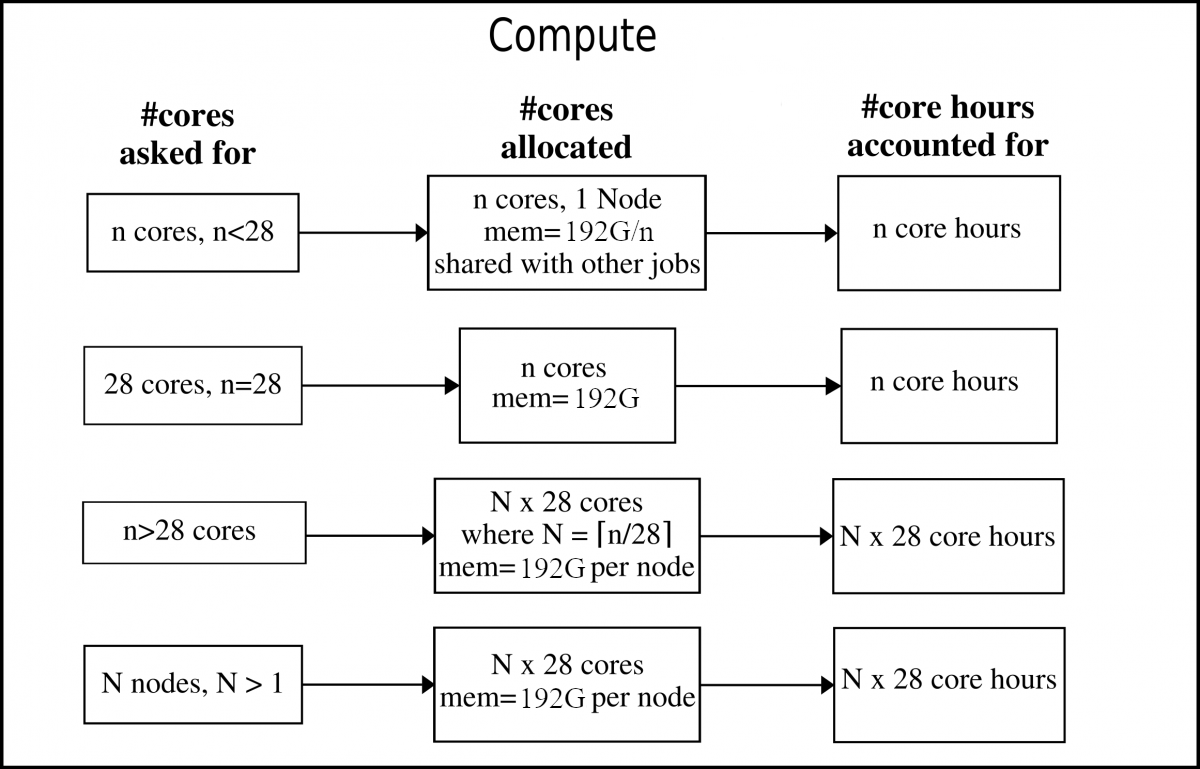
\includegraphics[width=9cm]{figures/Allocation-Kebnekaise-thin_skylake.png}
\end{center}
  \end{block}
}


\frame{\frametitle{The Batch System}\framesubtitle{Accounting, largemem nodes, Kebnekaise}

  \begin{block}{}
\begin{center}
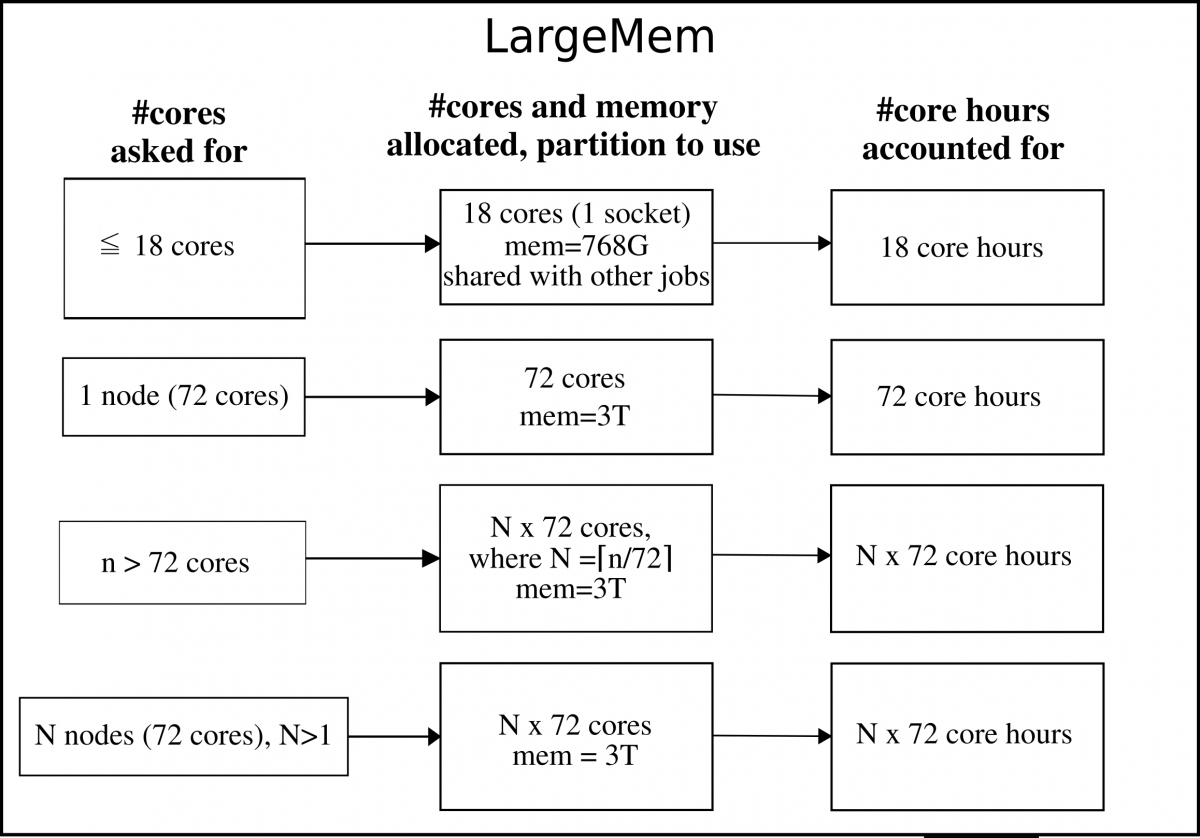
\includegraphics[width=10cm]{figures/Allocation-Kebnekaise-largemem_v3.png}
\end{center}
  \end{block}
}


\frame{\frametitle{The Batch System}\framesubtitle{Accounting, K80 GPU nodes, Kebnekaise.}

    \begin{block}{}
    \begin{footnotesize}
      The K80 GPU cards have 2 onboard compute engines (GK210 chips). Most GPU nodes have 2 K80s, placed together as 14 cores + 1 K80/socket. 4 GPU nodes have 4 K80 GPU cards. 
    \end{footnotesize}
  \end{block}
 
  \begin{block}{}
\begin{center}
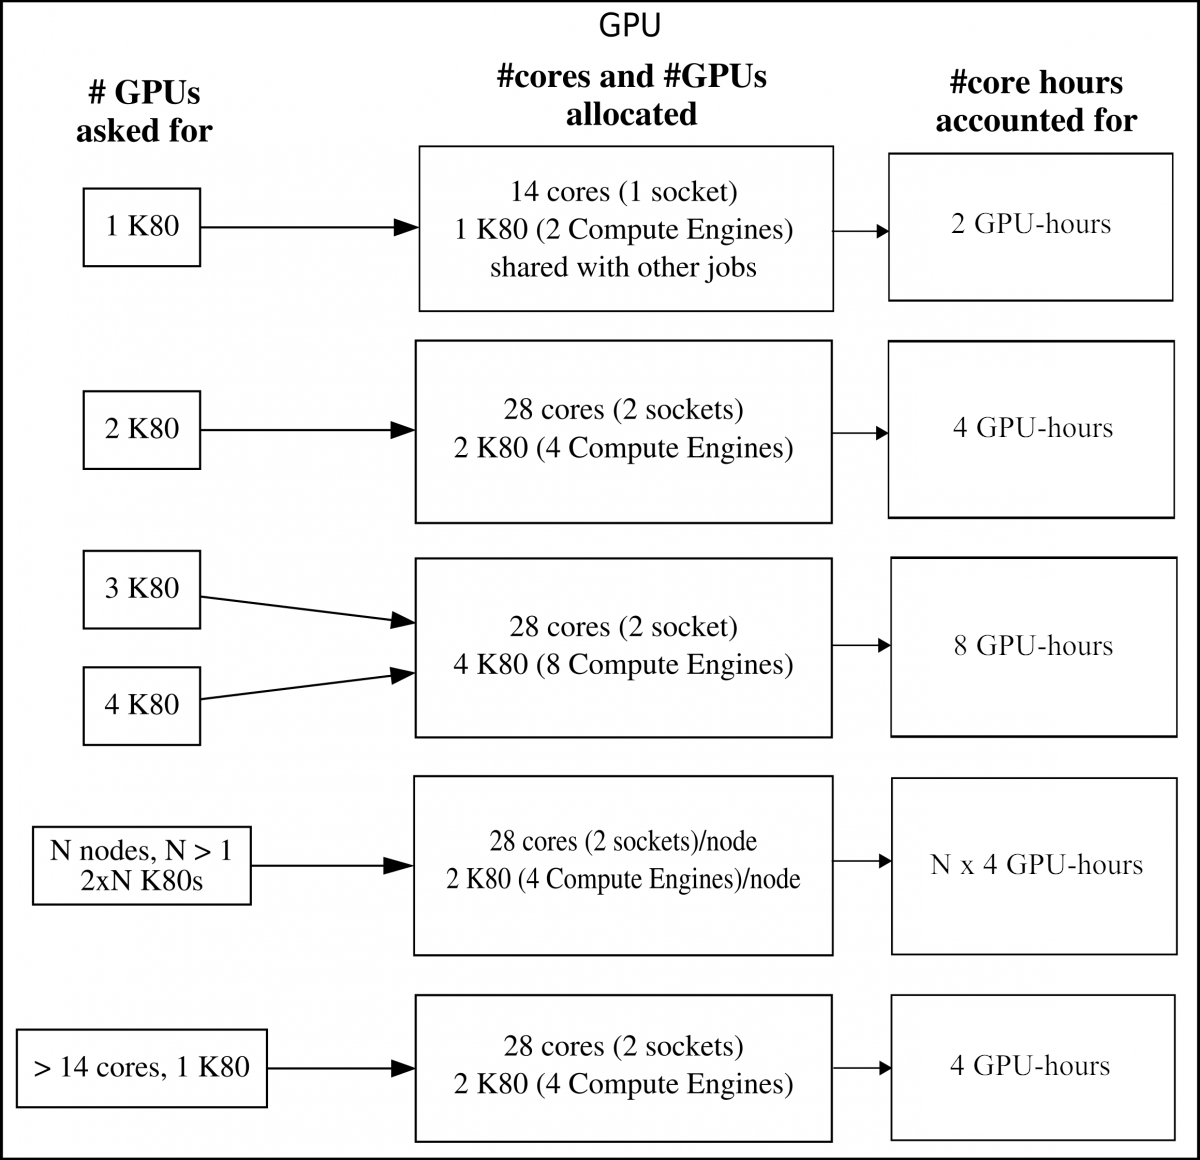
\includegraphics[width=5.8cm]{figures/K80-GPUs.png}
\end{center}
  \end{block}
}

\frame{\frametitle{The Batch System}\framesubtitle{Accounting, V100 GPU nodes, Kebnekaise.}

    \begin{block}{}
    \begin{scriptsize}
      Each V100 GPU accelerator card has 1 onboard compute engine (GV100 chip). They are placed together as 14 cores + 1 V100 on a socket (28 cores, 2 V100s per node).  
    \end{scriptsize}
  \end{block}
 
  \begin{block}{}
\begin{center}
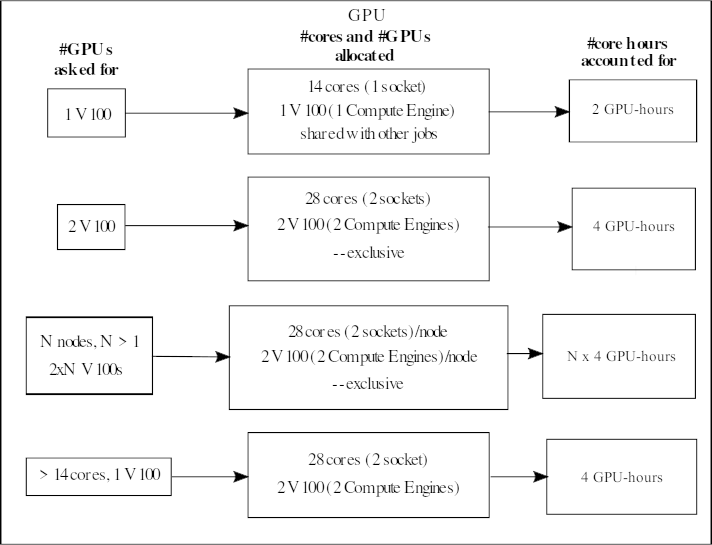
\includegraphics[width=6.8cm]{figures/V100-allocation-new.png}
\end{center}
  \end{block}
}

\frame{\frametitle{The Batch System}\framesubtitle{Accounting, A100 GPU nodes, Kebnekaise.}

    \begin{block}{}
    \begin{scriptsize}
      Each A100 GPU accelerator card has 1 onboard compute engine. The AMD Zen3 nodes have 2 CPUs sockets with 24 cores each, for a total of 48 cores, and 2 NVidia A100 GPUs. They are placed together as 24 cores + 1 A100 on a socket. 
    \end{scriptsize}
  \end{block}
 
  \begin{block}{}
\begin{center}
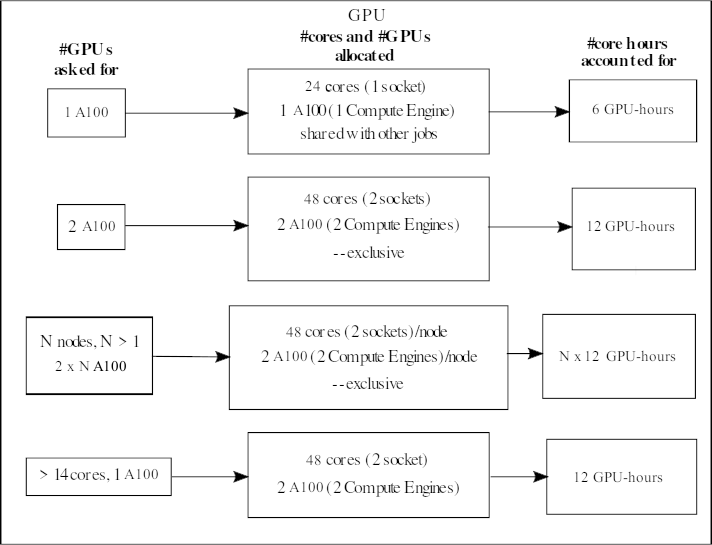
\includegraphics[width=6.8cm]{figures/A100-allocation.png}
\end{center}
  \end{block}
}

\frame{\frametitle{The Batch System (SLURM)}\framesubtitle{Useful Commands} 

  \begin{block}{}
    \begin{itemize}
      \begin{footnotesize}
      \item Submit job: \texttt{sbatch $<$jobscript$>$} 
      \item Get list of your jobs: \texttt{squeue -u $<$username$>$} 
      \item \texttt{srun $<$commands for your job/program$>$} 
      \item Check on a specific job: \texttt{scontrol show job $<$job id$>$} 
      \item Delete a specific job: \texttt{scancel $<$job id$>$}
      \item Delete all your own jobs: \texttt{scancel -u $<$user$>$}
      \item More detailed info about jobs: \\
      \end{footnotesize}
      \begin{scriptsize}      
        \texttt{sacct -l -j $<$jobid$>$ -o jobname,NTasks,nodelist,MaxRSS,MaxVMSize...}
      \end{scriptsize}
      \begin{itemize}
      \begin{footnotesize}
      \item More flags can be found with \texttt{man sacct}
      \item The output will be \textbf{very} wide. To view, use \\
        \texttt{sacct -l -j ....... | less -S} \\
        (makes it sideways scrollable, using the left/right arrow key)
        \end{footnotesize}
      \end{itemize}
      \begin{footnotesize}
      \item Web url with graphical info about a job: \texttt{job-usage $<$job-id$>$}
      \end{footnotesize}
    \end{itemize}
    Use \texttt{man sbatch, man srun, man ....} for more information
  \end{block}
}

\frame{\frametitle{The Batch System (SLURM)}\framesubtitle{Job Output} 

  \begin{block}{}
   \begin{itemize}
    \item  Output and errors in: \\ 
\texttt{slurm-$<$job id$>$.out}
    \item Look at it with vi, nano, emacs, cat, less...
    \item To get output and error files split up, you can give these flags in the submit script: \\ 
\texttt{\#SBATCH --error=job.\%J.err} \\ 
\texttt{\#SBATCH --output=job.\%J.out} 
   \end{itemize}
  \end{block}
}

 \frame{\frametitle{The Batch System (SLURM)}\framesubtitle{Using different parts of Kebnekaise} 

   \begin{block}{}
     \begin{scriptsize}
       \begin{itemize}
     \item Use the 'fat' nodes by adding this flag to your script: \\ 
 \texttt{\#SBATCH -p largemem} (separate resource) \\
     \item  Specifying Intel Broadwell, Intel Skylake, or AMD Zen3 CPUs: \\ 
 \texttt{\#SBATCH --constraint=broadwell} \\
 or \\
 \texttt{\#SBATCH --constraint=skylake} \\
 or \\
 \texttt{\#SBATCH --constraint=zen3} \\
     \item Using the GPU nodes (separate resource): \\ 
       \texttt{\#SBATCH --gres=gpu:$<$type-of-card$>$:x} where $<$type-of-card$>$ is either k80, v100, or a100 and x = 1, 2, or 4 (4 only for K80). \\
       \begin{itemize}
     \begin{scriptsize}
       \item In the case of the A100 GPU nodes, you also need to add a partition \\
         \texttt{\#SBATCH -p amd\_gpu}
     \end{scriptsize}
         \end{itemize}
       \item Use the AMD login node for correct modules and compilers for AMD Zen3 and A100 nodes: \\ \texttt{kebnekaise-amd-tl.hpc2n.umu.se} or \\\texttt{kebnekaise-amd.hpc2n.umu.se}
    \end{itemize}
 More on https://www.hpc2n.umu.se/documentation/guides/using\_kebnekaise
     \end{scriptsize}
   \end{block}
 }


\frame{\frametitle{The Batch System (SLURM)}\framesubtitle{Simple example, serial} 

  \begin{block}{}
    \justify
\begin{footnotesize}
Example: Serial job on Kebnekaise, compiler toolchain 'foss' 
\end{footnotesize}
  \end{block}

  \begin{block}{}
\begin{footnotesize}
\texttt{\#!/bin/bash} \\
\texttt{\# Project id - change to your own after the course!} \\
\texttt{\#SBATCH -A hpc2n2023-132} \\
\texttt{\# Asking for 1 core} \\
\texttt{\#SBATCH -n 1} \\
\texttt{\# Asking for a walltime of 5 min} \\ 
\texttt{\#SBATCH --time=00:05:00} \\ 
\vspace{3mm} 
\texttt{\# Purge modules before loading new ones in a script. } \\
\texttt{ml purge} \\ 
\texttt{ml foss/2021b} \\ 
\vspace{3mm}
\texttt{./my\_serial\_program}
\end{footnotesize}
  \end{block}

  \begin{block}{}
    \justify
\begin{footnotesize}
Submit with: \\
\texttt{sbatch $<$jobscript$>$} 
\end{footnotesize}
  \end{block}

}

\frame{\frametitle{The Batch System (SLURM)}\framesubtitle{Example, MPI C program} 

  \begin{block}{}
    \begin{footnotesize}
      \texttt{\#include $<$stdio.h$>$} \\
\texttt{\#include $<$mpi.h$>$} \\
\vspace{3mm} 
\texttt{int main (int argc, char *argv[]) {} \\ 
\vspace{3mm}
\texttt{int myrank, size;} \\ 
\vspace{3mm}
\texttt{MPI\_Init(\&argc, \&argv);} \\ 
\texttt{MPI\_Comm\_rank(MPI\_COMM\_WORLD, \&myrank);} \\ 
\texttt{MPI\_Comm\_size(MPI\_COMM\_WORLD, \&size);} \\ 
\vspace{3mm}
\texttt{printf("Processor \%d of \%d: Hello World!\textbackslash n", myrank, size);} \\ 
\vspace{3mm}
\texttt{MPI\_Finalize();}
\vspace{3mm}
\texttt{}}
    \end{footnotesize}
  \end{block}

} 


\frame{\frametitle{The Batch System (SLURM)}\framesubtitle{Simple example, parallel} 

  \begin{block}{}
    \justify
  \begin{footnotesize}
  Example: MPI job on Kebnekaise, compiler toolchain 'foss' 
  \end{footnotesize}
\end{block}

  \begin{block}{}
\begin{footnotesize}
\texttt{\#!/bin/bash} \\
\texttt{\#SBATCH -A hpc2n2023-132} \\
\texttt{\#SBATCH -n 14} \\
\texttt{\#SBATCH --time=00:05:00} \\ 
\texttt{\#\#SBATCH --exclusive} \\ 
\texttt{\#SBATCH --reservation=intro-cpu} \\ 
\vspace{3mm} 
\texttt{module purge} \\ 
\texttt{ml foss/2021b} \\ 
\vspace{3mm}
\texttt{srun ./my\_parallel\_program}
\end{footnotesize}
  \end{block}

}


\begin{frame}[fragile]\frametitle{The Batch System (SLURM)}\framesubtitle{Simple example, output} 

  \begin{block}{}
    \justify
Example: Output from a MPI job on Kebnekaise, run on 14 cores (one NUMA island)
  \end{block}

  \begin{block}{}
\begin{tiny}
\begin{verbatim}
b-an01 [~/slurm]$ cat slurm-15952.out 

The following modules were not unloaded:
   (Use "module --force purge" to unload all):

  1) systemdefault   2) snicenvironment
Processor 12 of 14: Hello World!
Processor 5 of 14: Hello World!
Processor 9 of 14: Hello World!
Processor 4 of 14: Hello World!
Processor 11 of 14: Hello World!
Processor 13 of 14: Hello World!
Processor 0 of 14: Hello World!
Processor 1 of 14: Hello World!
Processor 2 of 14: Hello World!
Processor 3 of 14: Hello World!
Processor 6 of 14: Hello World!
Processor 7 of 14: Hello World!
Processor 8 of 14: Hello World!
Processor 10 of 14: Hello World!
\end{verbatim}
\end{tiny}
  \end{block}

\end{frame}



\frame{\frametitle{The Batch System (SLURM)}\framesubtitle{Starting more than one serial job in the same submit file} 

  \begin{block}{}
\begin{small}
\texttt{\#!/bin/bash} \\
\texttt{\#SBATCH -A hpc2n2023-132} \\
\texttt{\#SBATCH -n 5} \\
\texttt{\#SBATCH --time=00:15:00} \\ 
\vspace{3mm} 
\texttt{module purge} \\ 
\texttt{ml foss/2021b} \\ 
\vspace{3mm}
\texttt{srun -n 1 ./job1.batch \&} \\ 
\texttt{srun -n 1 ./job2.batch \&} \\ 
\texttt{srun -n 1 ./job3.batch \&} \\ 
\texttt{srun -n 1 ./job4.batch \&} \\ 
\texttt{srun -n 1 ./job5.batch } \\
\texttt{wait} \\
\end{small}
  \end{block}

} 

\frame{\frametitle{The Batch System (SLURM)}\framesubtitle{Multiple Parallel Jobs Sequentially} 

  \begin{block}{}
\begin{scriptsize}
\texttt{\#!/bin/bash} \\
\texttt{\#SBATCH -A hpc2n2023-132} \\
\texttt{\#SBATCH -c 28} \\
\texttt{\# Remember to ask for enough time for all jobs to complete} \\ 
\texttt{\#SBATCH --time=02:00:00} \\ 
\vspace{3mm} 
\texttt{module purge} \\ 
\texttt{ml foss/2021b} \\ 
\vspace{3mm}
\texttt{\# Here 14 tasks with 2 cores per task. Output to file.} \\
\texttt{\# Not needed if your job creates output in a file} \\ 
\texttt{\# I also copy the output somewhere else and then run} \\
\texttt{\# another executable...} \\
\vspace{3mm}
\texttt{srun -n 14 -c 2 ./a.out > myoutput1 2>\&1} \\ 
\texttt{cp myoutput1 /pfs/nobackup/home/u/username/mydatadir} \\ 
\texttt{srun -n 14 -c 2 ./b.out > myoutput2 2>\&1} \\ 
\texttt{cp myoutput2 /pfs/nobackup/home/u/username/mydatadir} \\ 
\texttt{srun -n 14 -c 2 ./c.out > myoutput3 2>\&1} \\
\texttt{cp myoutput3 /pfs/nobackup/home/u/username/mydatadir} \\
\end{scriptsize}
  \end{block}

} 



\frame{\frametitle{The Batch System (SLURM)}\framesubtitle{Multiple Parallel Jobs Simultaneously} 

\begin{footnotesize}
Make sure you ask for enough cores that all jobs can run at the same time, and have enough memory. Of course, this will also work for serial jobs - just remove the srun from the command line.
\end{footnotesize} 

  \begin{block}{}
\begin{footnotesize}
\texttt{\#!/bin/bash} \\
\texttt{\#SBATCH -A hpc2n2023-132} \\
\texttt{\# Total number of cores the jobs need} \\
\texttt{\#SBATCH -n 56} \\
\texttt{\# Remember to ask for enough time for all of the jobs to} \\
\texttt{\# complete, even the longest} \\ 
\texttt{\#SBATCH --time=02:00:00} \\ 
\vspace{3mm} 
\texttt{module purge} \\ 
\texttt{ml foss/2021b} \\ 
\vspace{3mm}
\texttt{srun -n 14 --cpu\_bind=cores ./a.out \&} \\ 
\texttt{srun -n 28 --cpu\_bind=cores ./b.out \&} \\ 
\texttt{srun -n 14 --cpu\_bind=cores ./c.out \&} \\ 
\texttt{...} \\ 
\texttt{wait} \\
\end{footnotesize}
  \end{block}

} 


\frame{\frametitle{The Batch System (SLURM)}\framesubtitle{GPU Job - V100} 

  \begin{block}{}
\begin{footnotesize}
\texttt{\#!/bin/bash} \\
\texttt{\#SBATCH -A hpc2n2023-132} \\
\texttt{\# Expected time for job to complete}  \\ 
\texttt{\#SBATCH --time=00:10:00} \\
\texttt{\# Number of GPU cards needed. Here asking for 2 V100 cards} \\
\texttt{\#SBATCH --gres=v100:2} \\
\vspace{3mm} 
\texttt{module purge} \\
\texttt{\# Change to modules needed for your program} \\ 
\texttt{ml fosscuda/2021b} \\ 
\vspace{3mm}
\texttt{./my-cuda-program} \\
\end{footnotesize}
  \end{block}

}


\frame{\frametitle{The Batch System (SLURM)}\framesubtitle{GPU Job - A100} 

  \begin{block}{}
\begin{footnotesize}
\texttt{\#!/bin/bash} \\
\texttt{\#SBATCH -A hpc2n2023-132} \\
\texttt{\# Expected time for job to complete}  \\ 
\texttt{\#SBATCH --time=00:10:00} \\
\texttt{\# Adding the partition for the A100 GPUs} \\
\texttt{\#SBATCH -p amd\_gpu} \\ 
\texttt{\# Number of GPU cards needed. Here asking for 2 A100 cards} \\ 
\texttt{\#SBATCH --gres=a100:2} \\
\vspace{3mm} 
\texttt{module purge} \\
\texttt{\# Change to modules needed for your software - remember to login} \\
\texttt{\# to kebnekaise-amd.hpc2n.umu.se or} \\
\texttt{\# kebnekaise-amd-tl.hpc2n.umu.se login node to see availability} \\
\texttt{ml CUDA/11.7.0} \\ 
\vspace{3mm}
\texttt{./my-cuda-program} \\
\end{footnotesize}
  \end{block}

}


\frame{\frametitle{Important information}

  \begin{block}{}
    \begin{itemize}
      \begin{small}
      \item The course project has the following project ID: hpc2n2023-132
      \item In order to use it in a batch job, add this to the batch script:
        \begin{itemize}
          \begin{small}
          \item \#SBATCH -A hpc2n2023-132
          \end{small}
        \end{itemize}
      \item There is one A100 GPU node reserved for the course, in order to let us run small GPU examples without having to wait for too long.
      \item You can ONLY use the reservation when adding \texttt{\#SBATCH -p amd\_gpu} and \texttt{\#SBATCH --gres=a100:x (for x=1,2)}. 
      \item The reservation is ONLY valid during the course:
        \begin{itemize}
          \begin{small}
          \item intro-gpu \\ (add with \#SBATCH --reservation=intro-gpu)
          \end{small}
        \end{itemize}
      \item We have a storage project linked to the compute project. It is hpc2n2023-132. You find it in /proj/nobackup/hpc2n2023-132. Remember to create your own directory under it.
      \end{small}
    \end{itemize}
  \end{block}

}

\frame{\frametitle{Questions and support}

  \begin{block}{}
    \textbf{Questions?} Now: Ask me or one of the other support or application experts present. 

    \vspace{0.5cm}
    OR 
    \vspace{0.5cm}

    \begin{itemize}
    \item Documentation: \texttt{https://www.hpc2n.umu.se/support}
    \item Support questions to: \texttt{https://supr.naiss.se/support/} or \texttt{support@hpc2n.umu.se}
    \end{itemize}
  \end{block}

}

\end{document}






